\chapter{Теоретические сведения}
\label{ch:theory}

\section{Архитектура клиент-серверного веб-приложения}

Современное веб-приложение строится по схеме <<\,клиент~—~сервер\,>>
с чётким разделением ответственности. \textbf{Сервер} (бэкенд) хранит
данные, реализует бизнес-логику и предоставляет программный интерфейс
— \textbf{API}. \textbf{Клиент} (фронтенд) исполняется в браузере
пользователя, отвечает за интерфейс и обращается к серверу за данными.

В проекте применяется модель \textbf{одностраничного приложения}
(\textit{Single Page Application}, SPA): браузер один раз загружает
клиентский код, а далее не перезагружает страницу целиком — при
переходах он лишь запрашивает данные у API и перерисовывает нужные
части интерфейса. Такой подход даёт отзывчивый интерфейс и снимает с
сервера задачу генерации HTML.

Взаимодействие клиента и сервера идёт по единому каналу
\textbf{REST-API} поверх HTTP: регистрация, вход, загрузка и удаление
видео, чтение ленты, получение метаданных конкретного ролика.

\section{Серверные технологии: Python, Django и REST Framework}

\textbf{Django} — высокоуровневый веб-фреймворк на языке Python. Он
предоставляет объектно-реляционное отображение (\textbf{ORM}) для
работы с базой данных через классы-модели, систему миграций схемы,
готовую панель администратора и подсистему аутентификации.

\textbf{Django REST Framework} (DRF) — надстройка над Django для
построения REST-API. Ключевые понятия DRF: \textit{сериализаторы},
описывающие преобразование объектов модели в JSON и обратно с
валидацией; \textit{представления} и \textit{наборы представлений}
(\texttt{ViewSet}), реализующие обработку запросов; \textit{маршрутизаторы},
автоматически строящие URL-адреса для типовых CRUD-операций.

Аутентификация построена на \textbf{JWT} (\textit{JSON Web Token}) —
подписанных сервером токенах, которые клиент хранит у себя и прикладывает
к каждому запросу в заголовке \texttt{Authorization}. Токен \textit{access}
короткоживущий (30~минут) и удостоверяет личность; токен \textit{refresh}
живёт дольше (7~дней) и служит для получения нового access-токена без
повторного входа. Библиотека \texttt{djangorestframework-simplejwt}
реализует выпуск и проверку токенов.

\section{Потоковая отдача видео и HTTP Range}

При просмотре ролика плеер не загружает весь файл целиком: ему хватает
части, соответствующей текущей позиции. Стандарт HTTP описывает для
этого заголовок \texttt{Range}: клиент в запросе указывает байтовый
диапазон, сервер отвечает кодом \texttt{206 Partial Content} и нужным
куском. Это позволяет начинать воспроизведение почти мгновенно и
перематывать к произвольной точке без полной загрузки.

В режиме разработки Django сам отдаёт медиа-файлы из каталога
\texttt{MEDIA\_ROOT}, в продакшене эту работу берёт на себя
обратный прокси Caddy и nginx-контейнер фронтенда — оба корректно
обрабатывают Range-запросы.

\section{Клиентские технологии: React и React Router}

\textbf{React} — библиотека для построения пользовательских
интерфейсов из \textit{компонентов} — переиспользуемых строительных
блоков со своим состоянием. React хранит виртуальное представление DOM
и при изменении состояния обновляет только изменившиеся узлы реального
дерева.

\textbf{React Router} реализует клиентскую маршрутизацию: сопоставляет
адрес в строке браузера с компонентом-страницей без перезагрузки.
Сборку и среду разработки обеспечивает \textbf{Vite} — быстрый
сборщик с горячей заменой модулей.

\section{Макет интерфейса в Figma}

\textbf{Figma} — браузерный редактор интерфейсов. До начала разработки
в Figma спроектирован макет интерфейса видеохостинга: лента видео,
экраны регистрации и входа, страница просмотра, личный профиль
(рисунок~\ref{fig:figma}). Параллельно проработана дизайн-система —
поля ввода, кнопки, карточки видео и сообщений, — переиспользуемая на
всех экранах.

Дизайн-токены (цвета, типографика, отступы, скругления) вынесены в
один CSS-файл; правка одной строки в нём меняет соответствующий
параметр сразу во всём интерфейсе. Структура экранов и состав
компонентов перенесены из макета в код напрямую. Конкретная схема
авторизации — вход по имени пользователя и паролю, гостевые аккаунты —
описана в главе~\ref{ch:practice}.

\begin{figure}[h!]
  \centering
  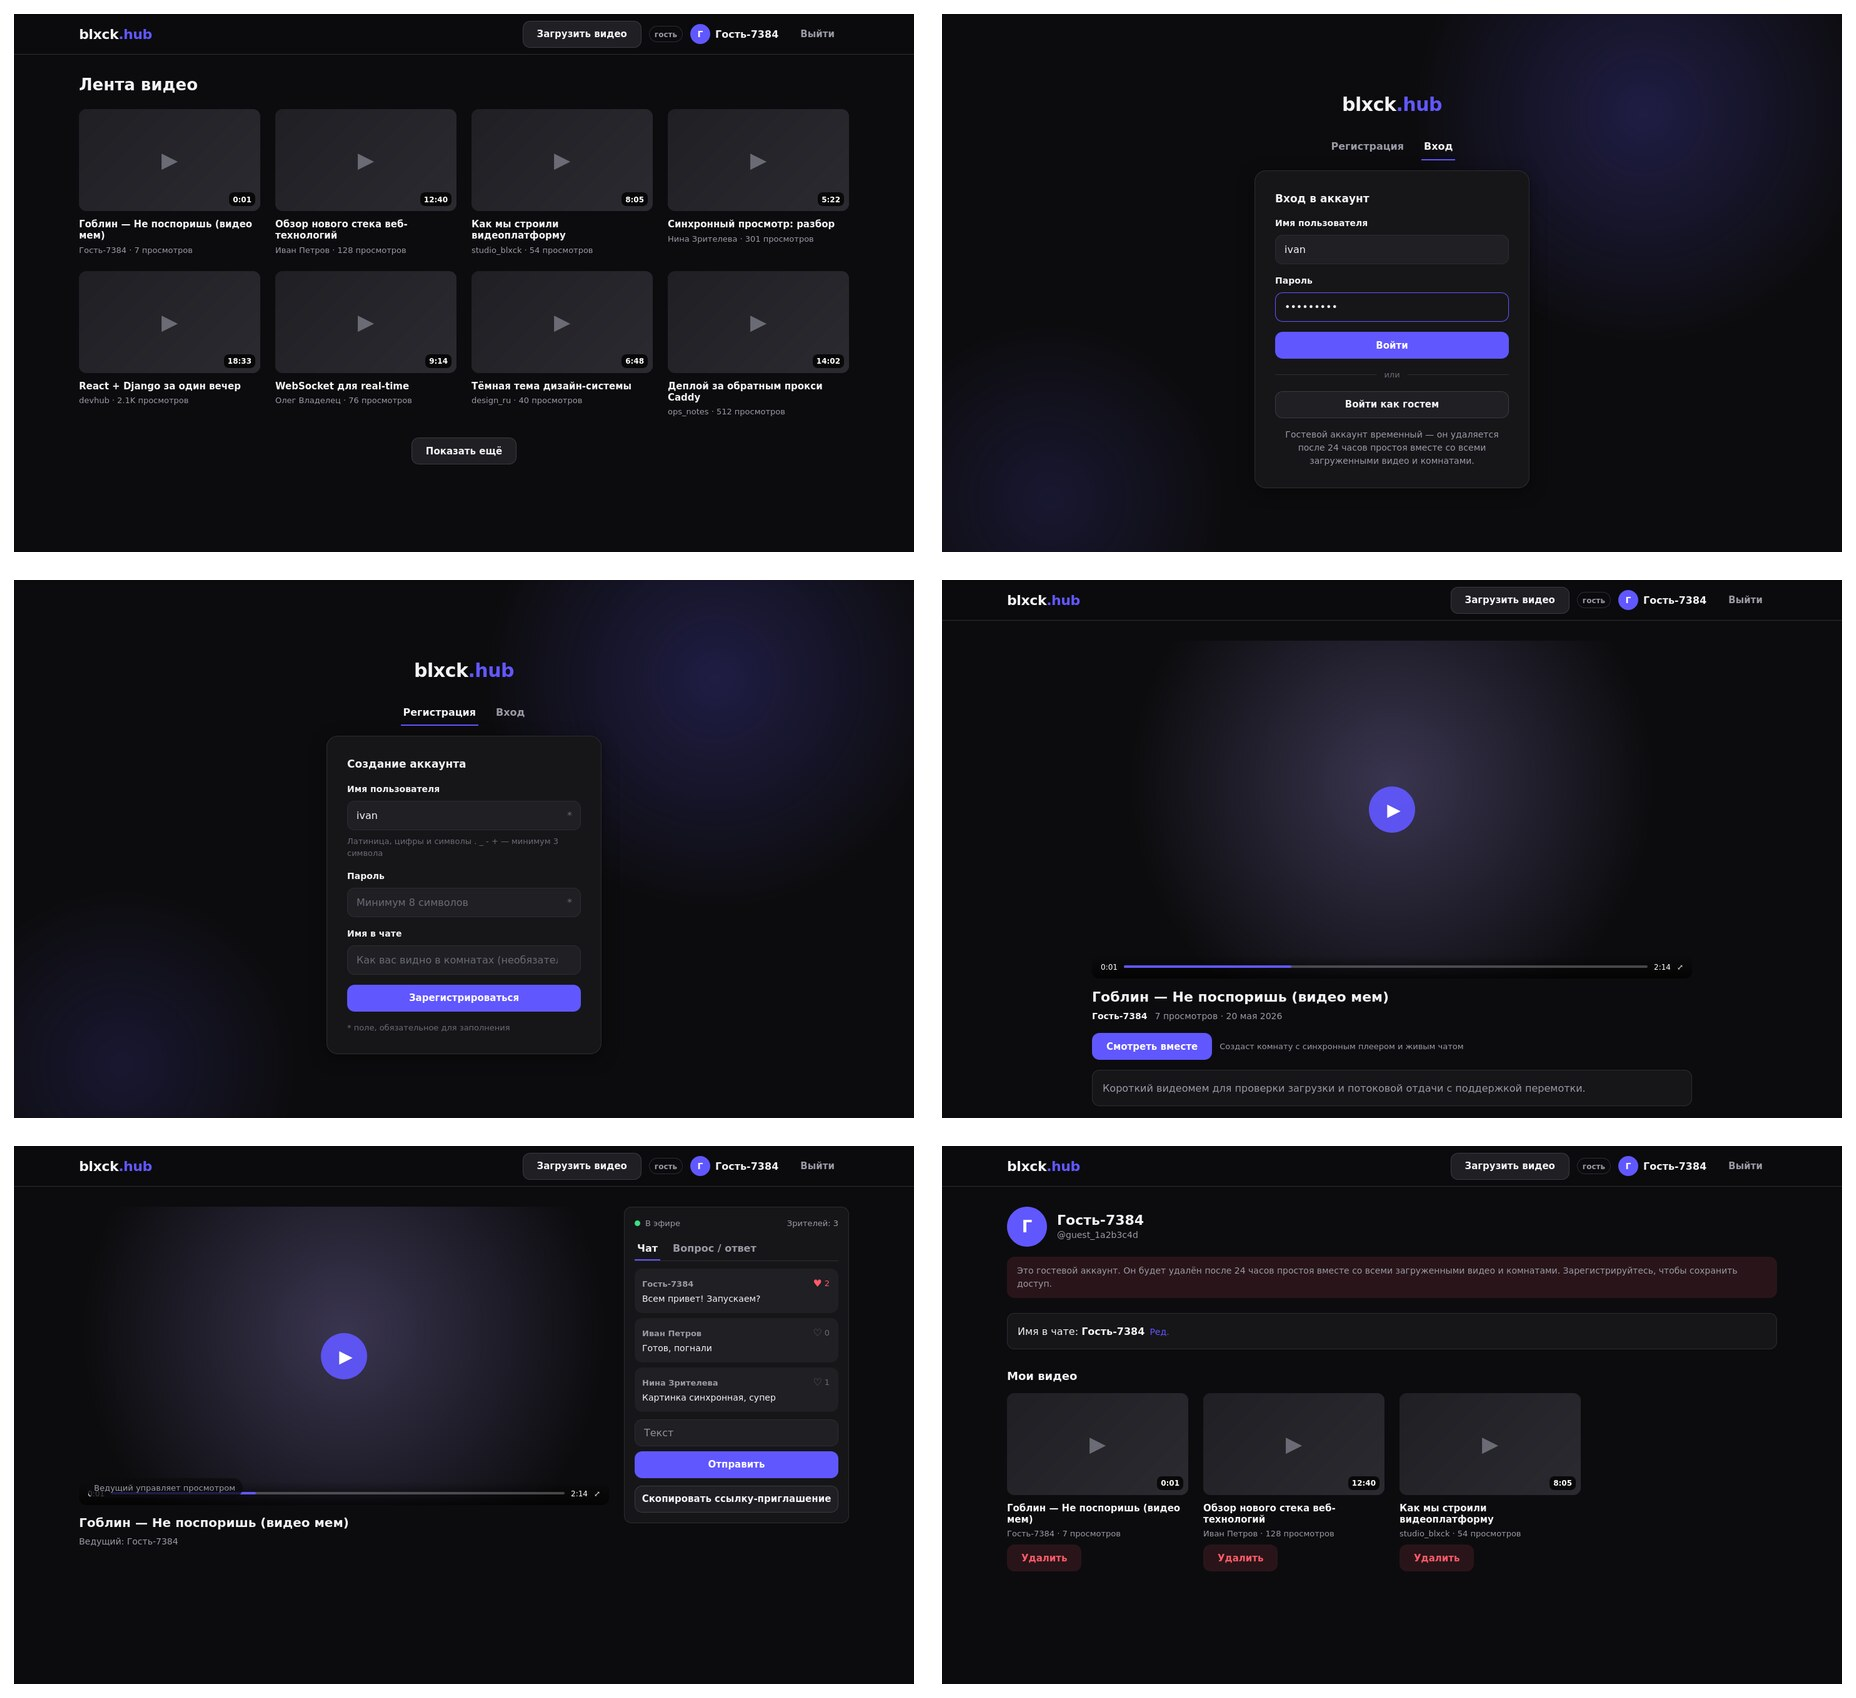
\includegraphics[width=\textwidth]{img/01_figma_design}
  \caption{Макет интерфейса видеохостинга в Figma}
  \label{fig:figma}
\end{figure}

\endinput
